% Options for packages loaded elsewhere
\PassOptionsToPackage{unicode}{hyperref}
\PassOptionsToPackage{hyphens}{url}
%
\documentclass[
]{article}
\usepackage{amsmath,amssymb}
\usepackage{lmodern}
\usepackage{iftex}
\ifPDFTeX
  \usepackage[T1]{fontenc}
  \usepackage[utf8]{inputenc}
  \usepackage{textcomp} % provide euro and other symbols
\else % if luatex or xetex
  \usepackage{unicode-math}
  \defaultfontfeatures{Scale=MatchLowercase}
  \defaultfontfeatures[\rmfamily]{Ligatures=TeX,Scale=1}
\fi
% Use upquote if available, for straight quotes in verbatim environments
\IfFileExists{upquote.sty}{\usepackage{upquote}}{}
\IfFileExists{microtype.sty}{% use microtype if available
  \usepackage[]{microtype}
  \UseMicrotypeSet[protrusion]{basicmath} % disable protrusion for tt fonts
}{}
\makeatletter
\@ifundefined{KOMAClassName}{% if non-KOMA class
  \IfFileExists{parskip.sty}{%
    \usepackage{parskip}
  }{% else
    \setlength{\parindent}{0pt}
    \setlength{\parskip}{6pt plus 2pt minus 1pt}}
}{% if KOMA class
  \KOMAoptions{parskip=half}}
\makeatother
\usepackage{xcolor}
\usepackage[margin=1in]{geometry}
\usepackage{graphicx}
\makeatletter
\def\maxwidth{\ifdim\Gin@nat@width>\linewidth\linewidth\else\Gin@nat@width\fi}
\def\maxheight{\ifdim\Gin@nat@height>\textheight\textheight\else\Gin@nat@height\fi}
\makeatother
% Scale images if necessary, so that they will not overflow the page
% margins by default, and it is still possible to overwrite the defaults
% using explicit options in \includegraphics[width, height, ...]{}
\setkeys{Gin}{width=\maxwidth,height=\maxheight,keepaspectratio}
% Set default figure placement to htbp
\makeatletter
\def\fps@figure{htbp}
\makeatother
\setlength{\emergencystretch}{3em} % prevent overfull lines
\providecommand{\tightlist}{%
  \setlength{\itemsep}{0pt}\setlength{\parskip}{0pt}}
\setcounter{secnumdepth}{-\maxdimen} % remove section numbering
\ifLuaTeX
  \usepackage{selnolig}  % disable illegal ligatures
\fi
\IfFileExists{bookmark.sty}{\usepackage{bookmark}}{\usepackage{hyperref}}
\IfFileExists{xurl.sty}{\usepackage{xurl}}{} % add URL line breaks if available
\urlstyle{same} % disable monospaced font for URLs
\hypersetup{
  pdftitle={Final Project: Predicting US Flight Delays using Flight Characteristics and Weather Data},
  pdfauthor={Oliver Ryder-Green},
  hidelinks,
  pdfcreator={LaTeX via pandoc}}

\title{Final Project: Predicting US Flight Delays using Flight
Characteristics and Weather Data}
\author{Oliver Ryder-Green}
\date{2022-11-27}

\begin{document}
\maketitle

\clearpage

\section{Introduction}

To paraphrase a well-known idiom, `nothing is certain but death, taxes,
and delayed flights.' Flight delays are an inconvenience that almost all
aviation passengers will experience at some point in their travels. Yet
the burden of flight delays is not the same for all passengers. In
particular, US passengers are not entitled to compensation for
delays\footnote{source:www.transportation.gov}. Yet, between 2013 and
2022, approximately one in every five flights from US airports was
delayed by at least 15 minutes\footnote{source:www.bts.gov}. With more
than 10 million scheduled passenger flights in the US each
year\footnote{source:www.faa.gov}, the cost to passengers of flight
delays is substantial. Indeed, the
\textit{Federal Aviation Administration} estimates that flight delays in
the US from 2016 to 2019 cost passengers US\$62.6billion in total. Short
of relying on airlines to inform them of expected delays, there is
little that US passengers can do to reliably avoid flight delays.
Therefore, I apply the classification methods discussed in class to
determine which factors inform flight departure delays for domestic
flights in the US.\\

Data from the \textit{Bureau of Transportation Statistics} illustrates
the prevalence of domestic flight delays. Among all US carriers, between
15--25\% of departures were delayed from 2010 to 2022. Among the top US
carriers\footnote{as measured by total number of flights serviced in 2010--2022.},
the proportion of delayed flights is persistently higher than average.
Evidently, some US carriers exhibit fewer than average flight delays
(e.g., Delta Airlines), but top US carriers tend to demonstrate more
frequent flight delays than the industry as a whole.

For US passengers, the fact that top US carriers experience more
frequent departure delays may be of interest in trying to avoid delays.
That said, more frequent delays at top airlines do not necessarily imply
more severe (i.e., costly) delays for passengers. The
\textit{Bureau of Transportation Statistics} data shows that, among all
US carriers, mean departure delay lengths were between 7 and 17 minutes
on average from 2010 to 2022. Unfortunately, top US carriers again
appear to perform worse than the industry as a whole. Without exception,
top US carriers exhibit longer-than-average delays at some point in the
period.

The \textit{Bureau of Transportation Statistics} data also highlights
that the frequency of delays varies by origin airport. In line with the
above, around one in every five flights from a US airport is delayed.
There are clearly some airports that persistently experience more
frequent delays, over 50\% of all flights in some cases, and some
airports that experience few or no delays.

Several factors may determine whether or not a flight is delayed and for
how long. The confluence of certain factors may also make delays more
likely or lengthy. Moreover, some factors are hard to observe or nearly
impossible to predict. The task of anticipating delays is, therefore,
extremely difficult for passengers. That said, the data above suggests
that some features that are readily observable for passengers may be
useful in avoiding delays. If passengers face a choice of carriers and
origin airports, they may be better able to avoid costly delays by
choosing those that feature less frequent and shorter delays. The aim of
this analysis is to identify factors that passengers might use to
anticipate delays.

\newpage 
\section{Data}

To identify factors that inform whether a flight is delayed on
departure, I use data from the
\textit{Bureau of Transportation Statistics' Airline On-Time Performance Data}\footnote{www.transtats.bts.gov/}
for January, March, September, and December in 2016, 2017, and 2018,
respectively. The flight data contains 8,777 observations on US domestic
flights and 21 features, such as the flight date, origin airport,
carrier, destination, distance, and other flight level characteristics.
I combine this data with weather data from
\textit{Weather Underground}\footnote{www.wunderground.com}. The weather
data contains weather observations, such as average temperature,
precipitation, and maximum wind speed, from corresponding airport
weather stations on flight departure dates.

\subsection{Compiling and Cleaning}

\subsubsection{Flight Data}

I manually download
\textit{Bureau of Transportation Statistics' Airline On-Time Performance Data}
for January, March, September, and December in 2016, 2017, and 2018,
respectively. I import the data and compile using Pandas in Python (see
corresponding Jupyter NB). The resulting dataset has 5,851,068
observations and 21 features. To make the dataset manageable, I draw a
random subset (fraction=0.0015) from each month-year sample. The
resulting dataset contains 8,777 observations.

\subsubsection{Weather Data}

I use web-scraping methods in Python (see corresponding Jupyter NB) to
acquire historical weather data from \textit{Weather Underground}. I use
airport codes corresponding to origin airports for departures in the
flight data to scrape historical weather data from airport weather
stations. I acquire observations on temperatures, precipitation, sea
level pressure, and max wind speed on the date of departure. The
resulting dataset contains 6,190 observations.

\subsubsection{Merged Data}

I merge the flight and weather data on the date of departure and origin
airport code. For the flight data, delays are identified as any flight
departing more than 15 minutes late: \texttt{DepDel15=1} if delayed and
\texttt{DepDel15=0} otherwise. Delays measured in minutes are given by
\texttt{DepDelay}. Since the supervised learning methods I utilise rely
on the assumption that \textbf{target variables} do not have missing
values, I drop observations if both \texttt{DepDel15} and
\texttt{DepDelay} are missing because such observations contain no
useful information for the analysis.

Since I am interested in predicting delays and delay lengths using
flight characteristics and weather observations, I consider the
proportion of missing values for these predictor variables. I find that
there are no missing observations in the flight data. However, around
70\% of observations have missing values for \texttt{Day.Average.Temp},
\texttt{High.Temp}, \texttt{Low.Temp}, \texttt{Max.Wind.Speed}, and
\texttt{Sea.Level.Pressure} (see Jupyter NB). Moreover, around 90\% of
observations have missing values for \texttt{Precipitation}. Dropping
observations missing weather data is costly in terms of observations.
Yet, the weather data is of interest in prediction and is likely
independent of many flight characteristics. I choose to omit
observations that have missing values for \texttt{Day.Average.Temp},
\texttt{High.Temp}, \texttt{Low.Temp}, \texttt{Max.Wind.Speed}, and
\texttt{Sea.Level.Pressure}.\\

Further omitting observations that have missing values for precipitation
may be discarding useful information: the correlation between
\texttt{DepDel15} and \texttt{Precipitation} (0.059) and between
\texttt{DepDelay} and \texttt{Precipitation} (0.026) are both
non-negligible, and; mean precipitation is higher for delayed departures
(0.446 inches) than for non-delayed departures (0.342 inches). Since
\texttt{Precipitation} is correlated with other weather observations, I
choose to impute missing values for \texttt{Precipitation} using
k-Nearest Neighbours on weather data. I optimise parameter \(k\) by
choosing \(k \in (0,100)\) to minimise the average MSE for in-sample
prediction across 50 random sub-samples of complete weather data (see
Jupyter NB). I impute missing values for \texttt{Precipitation} in the
merged dataset using \(k^*=2\). The resulting dataset has 2,693
observations and 27 features.

\subsection{Feature Engineering}

There is structure in the data that may be useful to exploit. For
instance, the data already splits flight dates into \texttt{Month},
\texttt{DayofMonth}, and \texttt{DayofWeek}, which may be relevant in
predicting flight delays if, for example, weekend flights are more prone
to delays. In a similar vein, I re-code \texttt{DepTimeBlk}, which gives
the astronomical time interval in which a departure is scheduled, as a
factor variable to be used in prediction. I likewise re-code
\texttt{ArrTimeBlk}. The variables \texttt{CRSDepTime} and
\texttt{CRSArrTime} give the scheduled departure and arrival times of a
flight in astronomical time. I find the difference in minutes between
scheduled departure and arrival times to categorise scheduled flight
lengths by hour in \texttt{SchFlTm}. The variable \texttt{Distance}
gives the flight distance in miles, I categorise flights by distance in
\texttt{DistGr} in intervals of 500 miles. I assign \texttt{InSt=1} if a
flight is within state and \texttt{InSt=0} otherwise using
\texttt{OriginStateName} and \texttt{DestStateName}. Finally, I use a
stricter definition of a departure delay than that of \texttt{DepDel15}.
I assign \texttt{Delayed=1} if \texttt{DepDelay>0} and
\texttt{Delayed=0} otherwise. The dataset used for the analysis contains
2,685 observations and 31
features\footnote{Note: I remove \texttt{Flights}, which gives the number of flights per flight journey, since it is equal to one for all observations and therefore containts no useful information.}.

\subsection{Summary}

In the data, the balance of departure delays is:

\begin{center}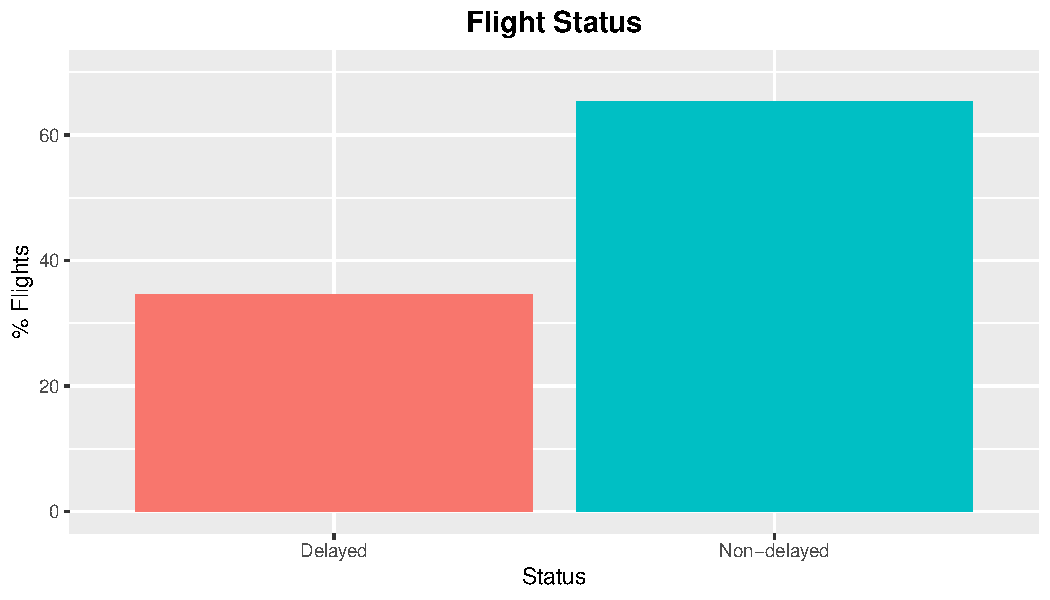
\includegraphics{Visualisation_Analysis_files/figure-latex/delay_plt-1} \end{center}

\newpage

The distribution of departure delay lengths
is\footnote{Early departures have negative delay lengths.}:

\begin{center}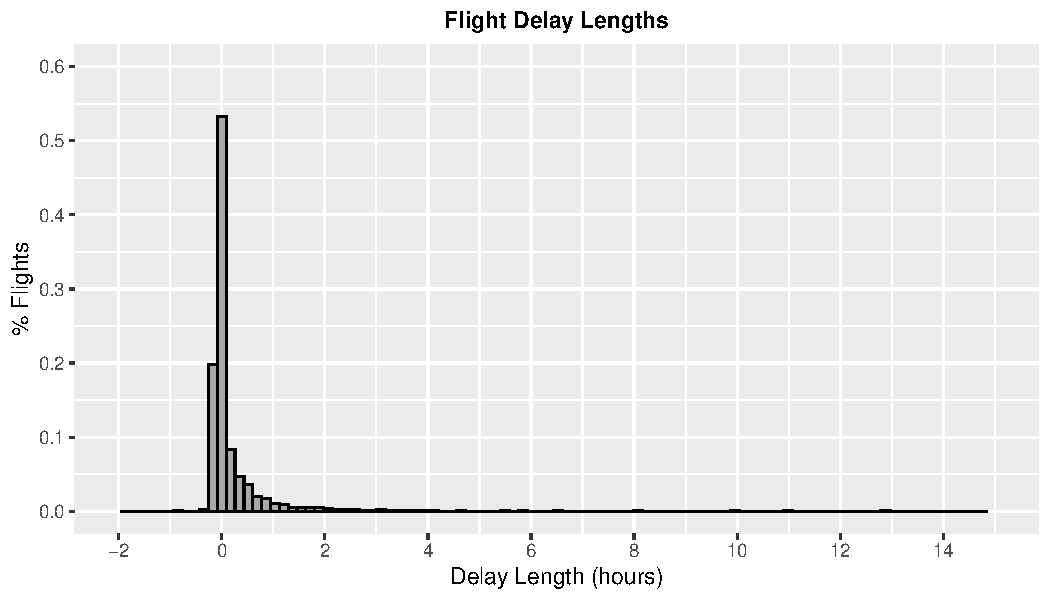
\includegraphics{Visualisation_Analysis_files/figure-latex/length_plt-1} \end{center}

I consider the features that may be useful in distinguishing between
delayed and non-delayed flights. Delayed flights tend to have longer
scheduled flight times:

\begin{center}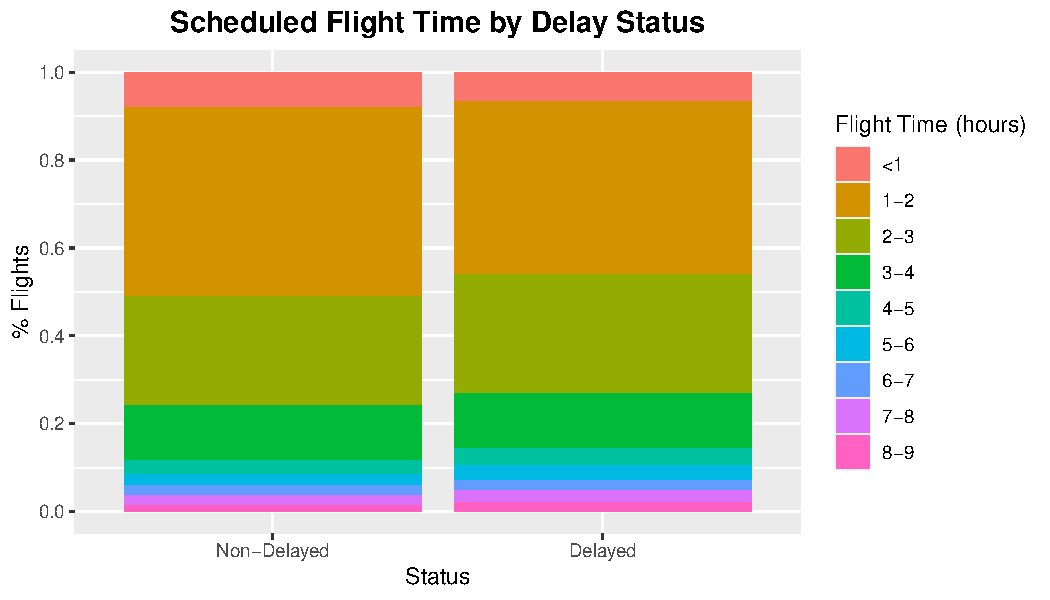
\includegraphics{Visualisation_Analysis_files/figure-latex/features_plt_6-1} \end{center}
\newpage

Accordingly, delayed flights tend to have greater flight distances:

\begin{center}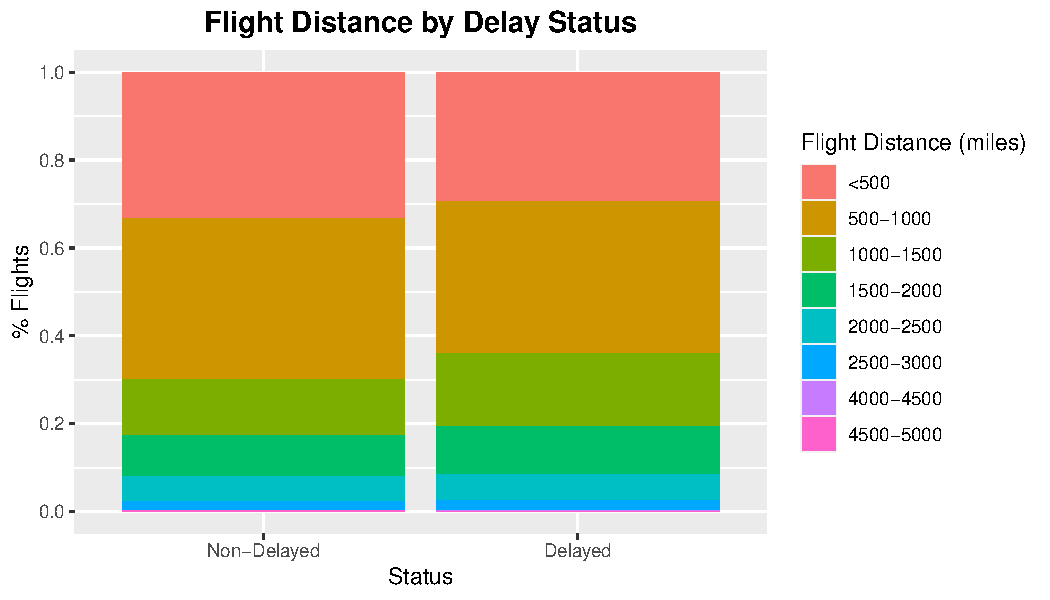
\includegraphics{Visualisation_Analysis_files/figure-latex/features_plt_7-1} \end{center}

Delayed flights tend to be scheduled to depart at later in the day:

\begin{center}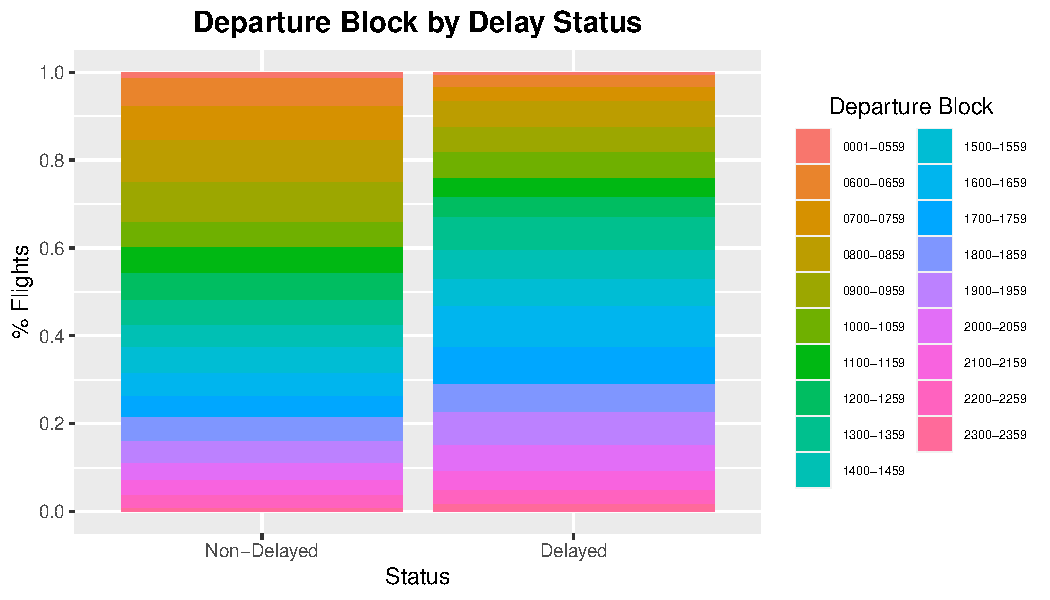
\includegraphics{Visualisation_Analysis_files/figure-latex/features_plt_8-1} \end{center}
\newpage

Delayed flights also tend to be scheduled to depart at later in the week
(i.e., Thursday and Friday):

\begin{center}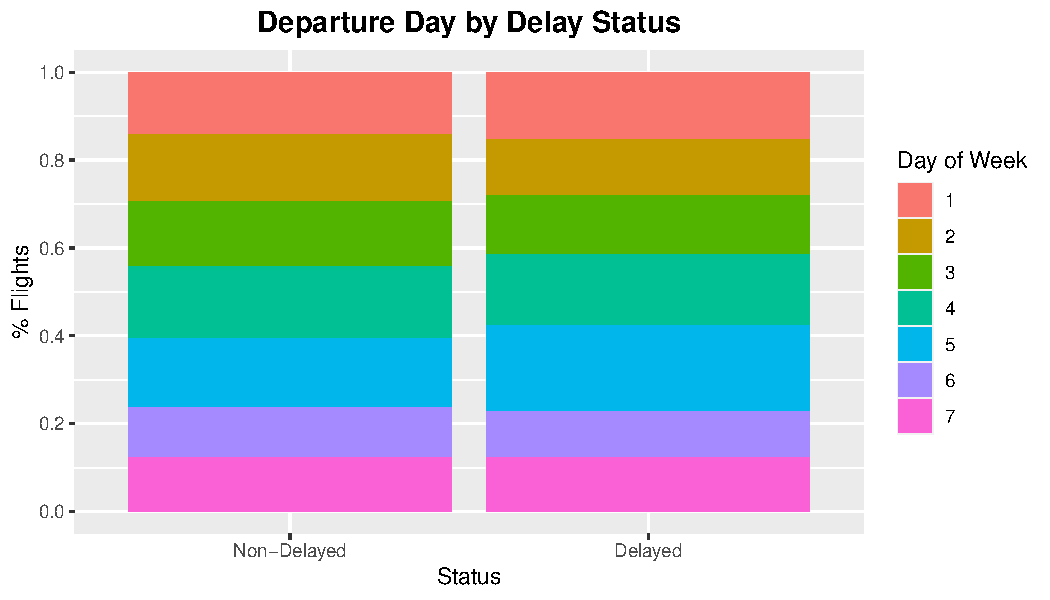
\includegraphics{Visualisation_Analysis_files/figure-latex/features_plt_9-1} \end{center}

Flight delays appear to coincide somewhat more frequently with colder
weather:

\begin{center}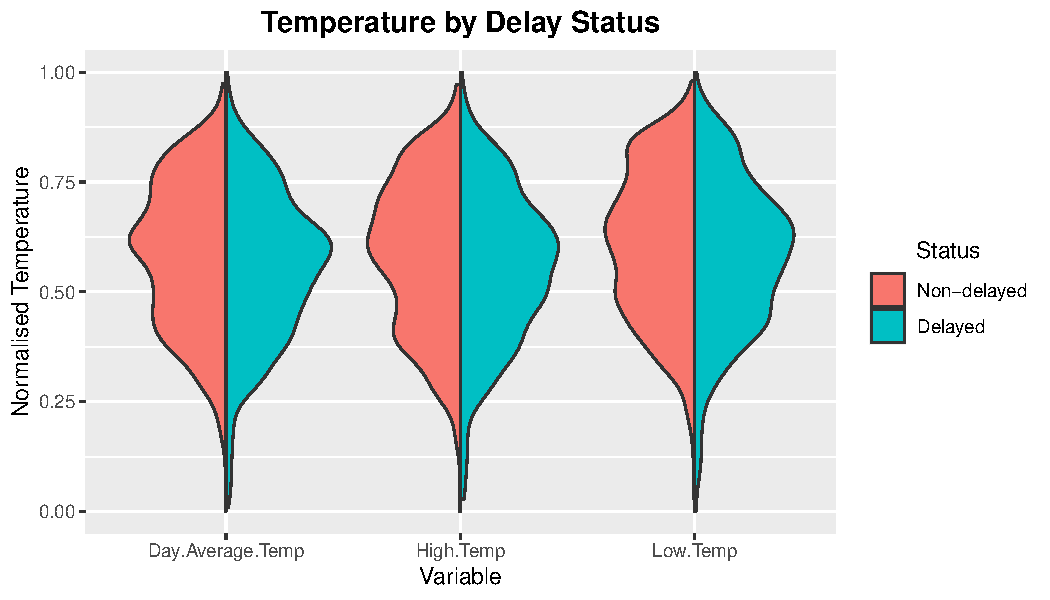
\includegraphics{Visualisation_Analysis_files/figure-latex/features_plt_10-1} \end{center}
\newpage

Flight delays appear to coincide somewhat more frequently with more
adverse
weather\footnote{note: the upper tails for \texttt{Max.Wind.Speed} and \texttt{Precipitation} belong to the distributions for delayed flights.}:

\begin{center}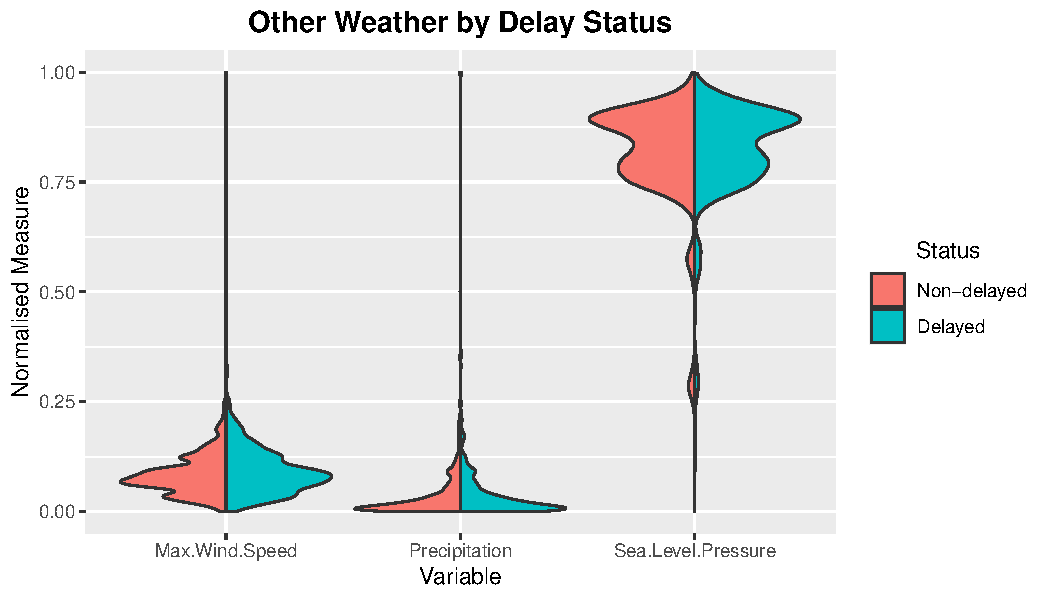
\includegraphics{Visualisation_Analysis_files/figure-latex/features_plt_11-1} \end{center}

\subsection{Methodology and Results}

\subsection{Conclusion}

Happy flying.

\end{document}
